In section \ref{section_tree_based_models}, it is explained how the learning algorithm of a decision tree works. Therefore, Figure \ref{fig:sigmoid_dtree} was used to visually interpret the predictions made by the model based on the dataset used to train the model and the internal structure of the model. At this point, it is a matter of keeping the gist of the visualization and additionally make use of the constraint validation results to create a visualization, which allows to further interpret the decision tree with respect to the user-defined constraints and explains predictions of the decision tree in suitable cases as demonstrated in section \ref{section_confusion_matrix_decomposition} and example \ref{Bsp:grouped_stacked_histogram}.

\paragraph{Frequency Distribution Tables to Summarize the Constraint Validation Results w.r.t. the Leaves of the Decision Tree} 

The frequency distribution tables introduced before lay the foundation to visualize the validation results. But they do not make use of the internal structure of the decision tree. To reflect the internal structure of the decision tree, each frequency distribution table will correspond to a node $n_{d,u}$ and the set of samples used to create the frequency distribution table is limited to $R_{d,u}$. As defined in section \ref{section_tree_based_models}, $R_{d,u}$ is the set of samples, which were used to decide, whether the node $n_{d,u}$ is going to be a split or a leaf node. Therefore, the resulting node visualization in Figure \ref{fig:sigmoid_dtree} (in the case of a regression task) and Figure \ref{motivating_example_decision_tree} (in the case of a classification task) made use of this limitation to show the effect these samples had on the decisions made for that node (e.g., the node type and parameters). This is what the visualization of a frequency distribution table using the constraint validation results of the samples $R_{d,u}$ should also achieve: \emph{Show the node relevant constraint validation results, to allow for interpretations of patterns in the data and predictions of the decision tree, leading to the internal structure of the decision tree}.

Formally, a grouping function is defined, which captures the mapping of indices of samples in the dataset to nodes in the decision tree according to the $R_{d,u}$ sets:

\begin{gather}
    \Gamma_\text{nodes}(n_{d,u}) = \{i \mid (x_i,t_i) \in R_{d,u}\}
\end{gather}

Using the new defined grouping function, the frequency distribution table to be used for the visualization of the leaf nodes, to summarize the constraint validation results, can be defined:
\begin{gather}
    \mathcal{F}_{G,C}(\Gamma_\text{nodes}(n_{d,u}),\Theta, \Gamma_\text{all}) \label{formula_single_constraint_leaf}\\
    COV_{G,\mathcal{C}}(\Gamma_\text{nodes}(n_{d,u}),\Theta,\Gamma_\text{all}) \label{formula_multiple_constraints_leaf}
\end{gather}
where $\Gamma_\text{all}$ corresponds to the function, which maps all samples to a single group.
As discussed in section \ref{section_visualizing_multiple_constraint_validation_results} for the visualization of the constraint validation results in case of multiple constraints, formula \ref{formula_single_constraint_leaf} has to be executed once per constraint or use the frequency distribution table showing the \glqq coverage\grqq{} of the constraint validation results by prioritizing them.

The procedure leads to a pie chart as shown in Figure \ref{fig:samples_for_indices_plot_3valued} (in the case of a single constraint) or Figure \ref{coverage_dataset} (in the case of multiple constraints and using coverage), or to a histogram as shown in Figure \ref{fig:class_per_constraints_samples_plot}. The latter one additionally uses $\Gamma_\text{predicted class}$, which does not makes sense for a leaf node, as the prediction will be constant for all samples visualized. However, $\Gamma_\text{ground truth class}$ can be used in case of classification. This way the plots in the leafs will show the distribution of the ground truth class as the leaves of Figure \ref{motivating_example_decision_tree} did. This modification additionally allows for interpretations analogue to section \ref{section_confusion_matrix_decomposition} (see Figure \ref{fig:decision_tree_node_gt_viz}). 

\begin{figure}
    \centering
    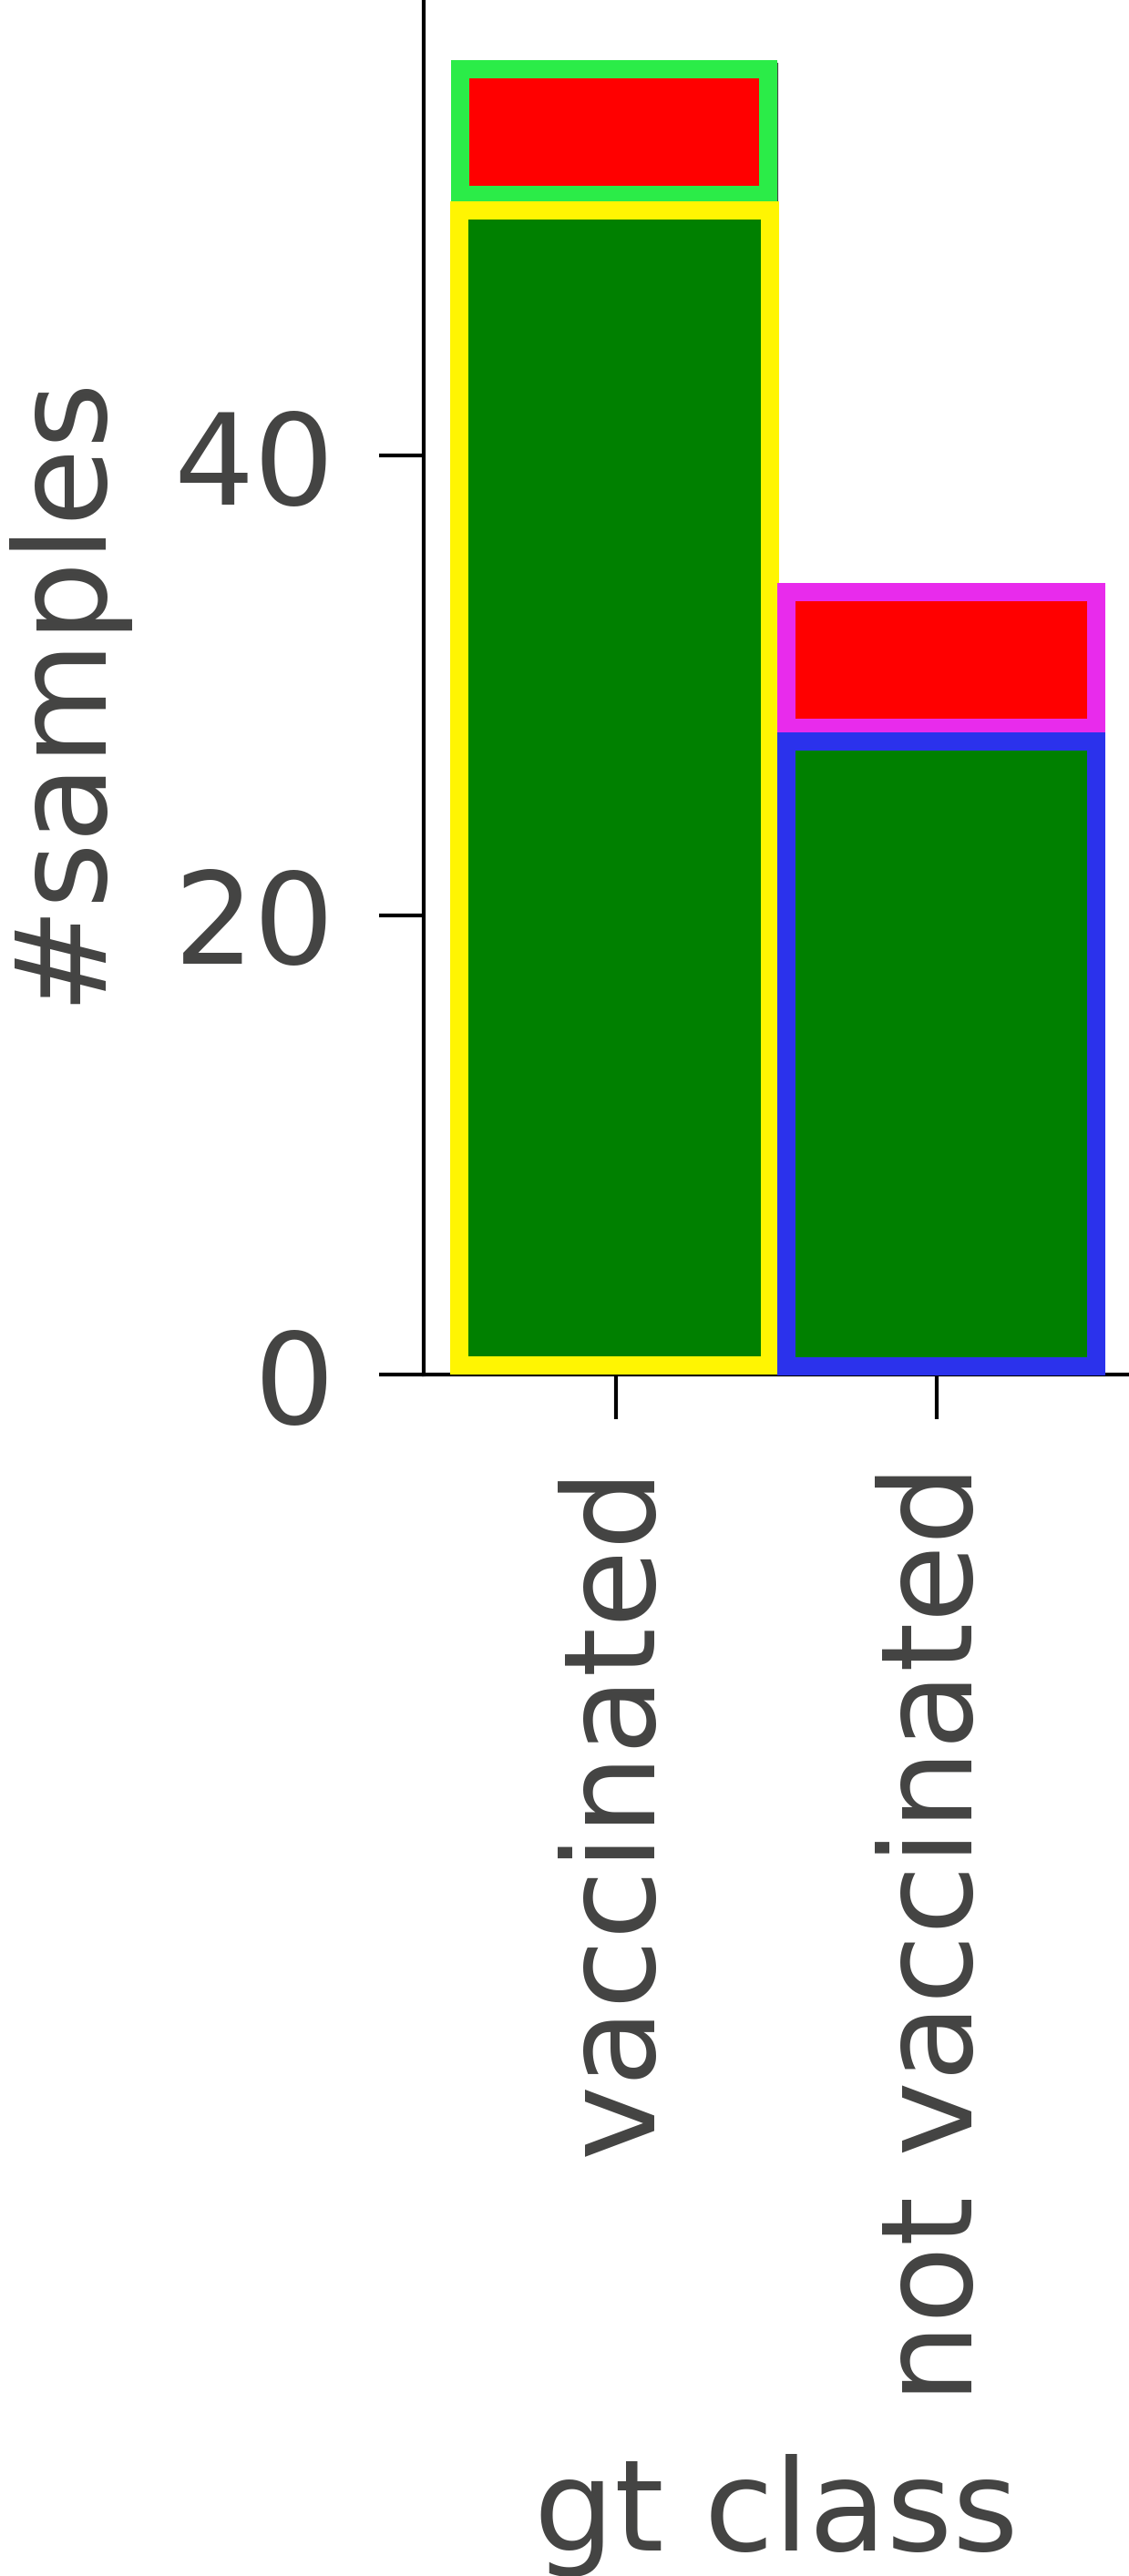
\includegraphics[width=0.2\textwidth]{images/visualizations/leaf_gt_viz.png}
    \caption{Decision Tree Node Visualization of the frequency distribution table using $\Gamma_\text{ground truth class}$. The border colors are chosen according to the interpretation from section \ref{section_confusion_matrix_decomposition}. The visualized leaf predicts the persons to be \emph{vaccinated}.}
    \label{fig:decision_tree_node_gt_viz}
\end{figure}


\paragraph{Frequency Distribution Tables to Summarize the Constraint Validation Results w.r.t. the Split Nodes of the Decision Tree} 

In a next step, frequency distribution tables should be created for the split-nodes, by extending the work done for the leaf nodes. As discussed in section \ref{section_tree_based_models}, figures \ref{motivating_example_decision_tree} and \ref{fig:sigmoid_dtree} use the split nodes, to show the marginal effect of the split feature on the ground truth. With respect to the constraint validation results, the goal is to \emph{show the marginal effect the split feature has on the constraint validation results, to be able to identify patterns in the data and predictions made by the decision tree}. To achieve the goal, a grouping function $\Gamma_\text{bins}^{f_k}$ is defined, which groups the samples to be visualized, according to their split feature value (e.g., the value of $f_k$):

\begin{gather}
    \Gamma_\text{bins}^{f_k}(b) = \left\{i \mid \exists (\mathbf{x}_i,t_i) \in D \land (b-1) * s \leq (\mathbf{x}_{i,k} - \textrm{min}) < b * s  \right\}
\end{gather}
where
\begin{align*}
    b & \in [1,...,B], \\
    \textrm{max} & = max(\{ \mathbf{x}_{i,k} \mid \exists t_i ~ (\mathbf{x}_i,t_i) \in D\}),\\
    \textrm{min} & = min(\{ \mathbf{x}_{i,k} \mid \exists t_i ~ (\mathbf{x}_i,t_i) \in D\}),\\
    s & = \frac{\textrm{max} - \textrm{min}}{B}
\end{align*}
and $B$ is the number of groups. 

Finally, the formulas needed to create the frequency distribution table per split node $n_{d,u}$ can be given, 
\begin{gather}
    \mathcal{F}_{G,C}(\Gamma_\text{nodes}(n_{d,u}),\Theta, \Gamma_\text{bins}^{f_k}) \label{formula_single_constraint_split}\\
    COV_{G,\mathcal{C}}(\Gamma_\text{nodes}(n_{d,u}),\Theta,\Gamma_\text{bins}^{f_k}) \label{formula_multiple_constraint_splits}
\end{gather}
where formula \ref{formula_single_constraint_split} is used in case of a single constraint $C$ and formula \ref{formula_multiple_constraint_splits} in case of a set of constraints $\mathcal{C}$. 

Figures \ref{motivating_example_decision_tree} and \ref{fig:sigmoid_dtree} both visualize the cuboid borders added by the corresponding split nodes to explain the set of samples used in the child nodes. The procedure leads to split nodes as used in Figure \ref{motivating_example_annotated_decision_tree} (in the case of a single constraint) and \ref{fig:decision_tree_split_node_marginal_effect_viz} (in the case of multiple constraint using coverage). The latter should emphasize the significance of summarizing the constraint validation results using coverage as the given procedure does not allow visualizing the constraint validation results of multiple constraints in a useful way, when showing the marginal effect of the split feature.

\begin{figure}
    \centering
    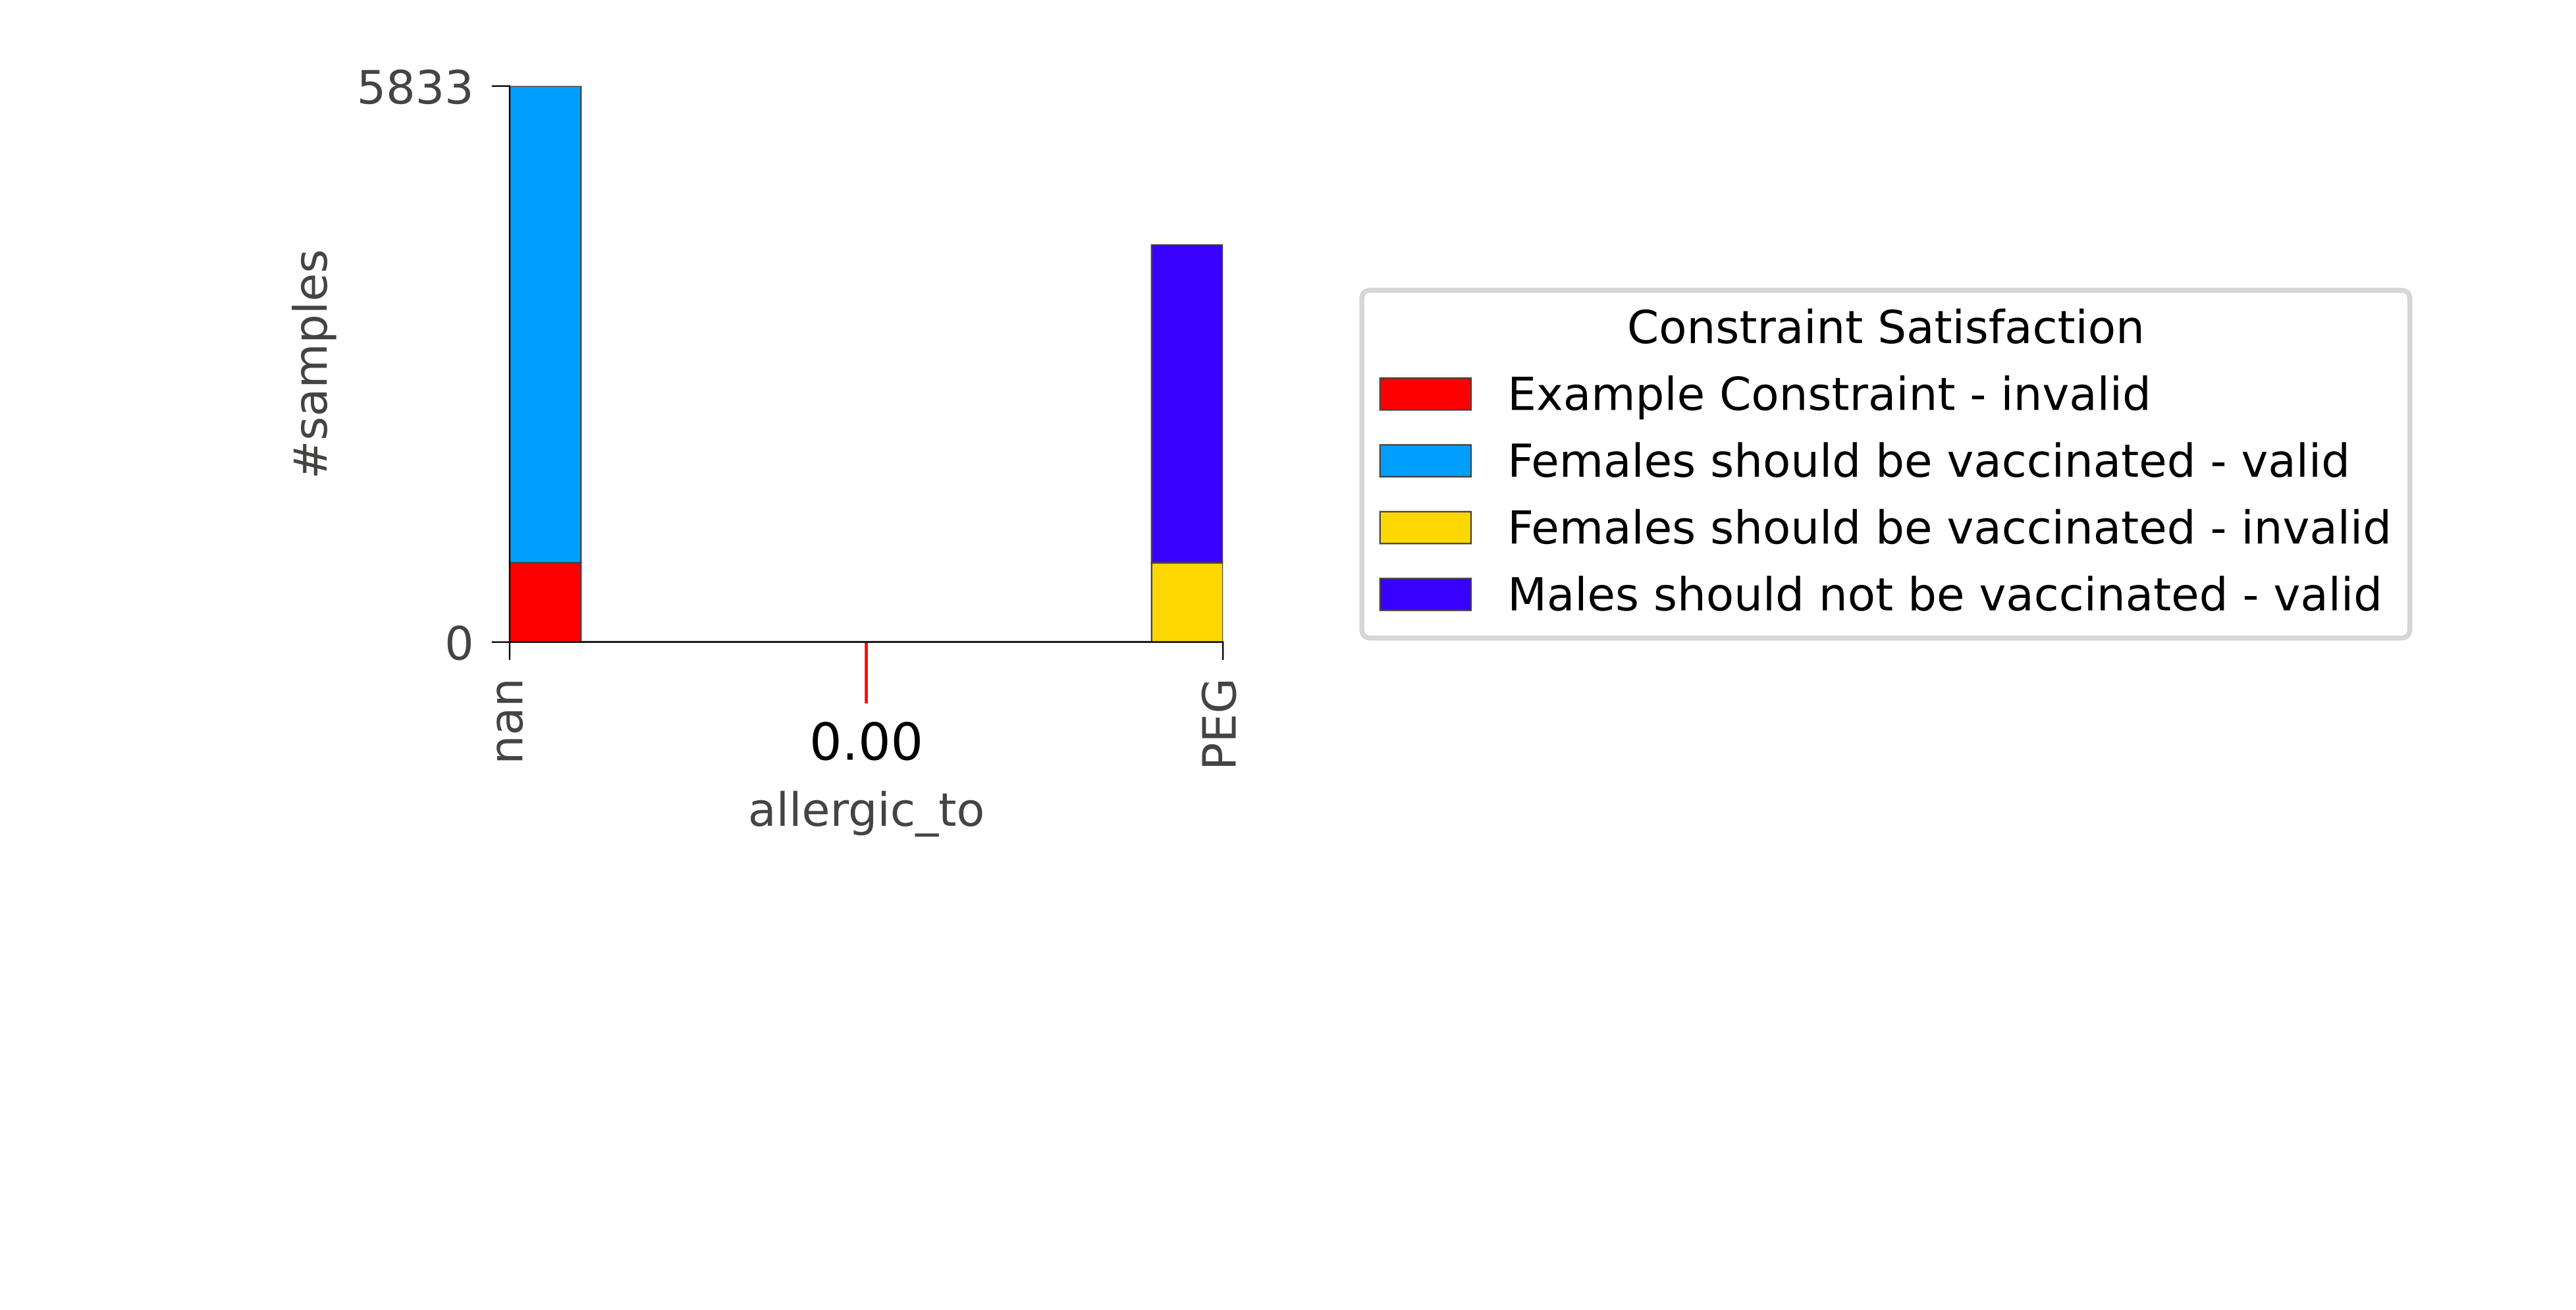
\includegraphics[trim=400 600 0 0, width=\textwidth]{images/visualizations/marginal_effect_split_node.png}  
    \caption{Summarizing validation results in bins given the allergic\_to split feature and marking the cuboid border added by the split node. The numerical values on the x-axis have been replaced with their corresponding categorical label, the cuboid border, however, can only be given numerical.}
    \label{fig:decision_tree_split_node_marginal_effect_viz}
\end{figure}



\paragraph{Composing the Visualizations}
Finally, all the visualizations of the different nodes can be composed analogue to figures \ref{motivating_example_decision_tree} and \ref{fig:sigmoid_dtree}. This now allows tracking the flow of the constraint validation results through the decision tree. To highlight the number of samples summarized in each visualization, the size of the visualizations per node are chosen proportional to the number of samples summarized.

\begin{Bsp}{Visualizing the Validation Results $\Theta$ given a Decision Tree $M_\theta$}{composing_the_annotated_decision_tree}
    Using the validation results of the example constraint given in Figure \ref{fig:validation_results_summary_theta}, the application of the formulas \ref{formula_single_constraint_split} and \ref{formula_single_constraint_leaf} can be seen in Figure \ref{motivating_example_annotated_decision_tree}. Borrowing the node enumeration from Figure \ref{motivating_example_decision_tree}, node $0$ and node $1$ are split nodes. Hence, formula \ref{formula_single_constraint_split} was applied, which allows to annotate the corresponding visualization with the cuboid borders associated with the \glqq allergic\_to\grqq{} and the \glqq pregnant\grqq{} feature. As a consequence of setting $D_{\text{idx}}$ to $\Gamma_\text{nodes}(n_{d,u})$ for all nodes $n_{d,u}$ and marking the cuboid borders, the flow of the validated and invalidated samples can be tracked from the root node into the leaves. For example, the invalidated samples can be tracked to occur only in the case of persons pregnant but not allergic to PEG. The leave nodes are based on the frequency distribution tables created with formula \ref{formula_single_constraint_leaf} and, therefore, do not show the distribution of the ground truth class.
    
    Using $\Gamma_\text{ground truth class}$ instead and making use of formulas \ref{formula_multiple_constraint_splits} and \ref{formula_multiple_constraints_leaf}, enables to visualize multiple constraints and additionally shows the distribution of the ground truth class in the leaves. The result of this procedure is depicted in Figure \ref{fig:multiple_constraints_gt_annotated_motivating_example_decision_tree}. The interpretations given in section \ref{section_confusion_matrix_decomposition} allow making statements about the leaves of the decision tree:
    \begin{enumerate}
        \item Not allergic persons which are not pregnant are classified correctly according to the constraint and to the ground truth data.
        \item Not allergic persons which are pregnant are classified correctly to the ground truth data. However, the classification violates the example constraint, which might imply overfitting, as will be seen later.
        \item Men allergic to PEG are classified correctly according to the constraints and to the ground truth data.
        \item Women allergic to PEG are classified incorrectly according to a constraint stating that females should be vaccinated. The decision was made on the basis of ground truth data.
    \end{enumerate}

    \captionsetup{type=htypei}
    \begin{minipage}[]{\linewidth}
            \vspace{1ex}
            \centering
            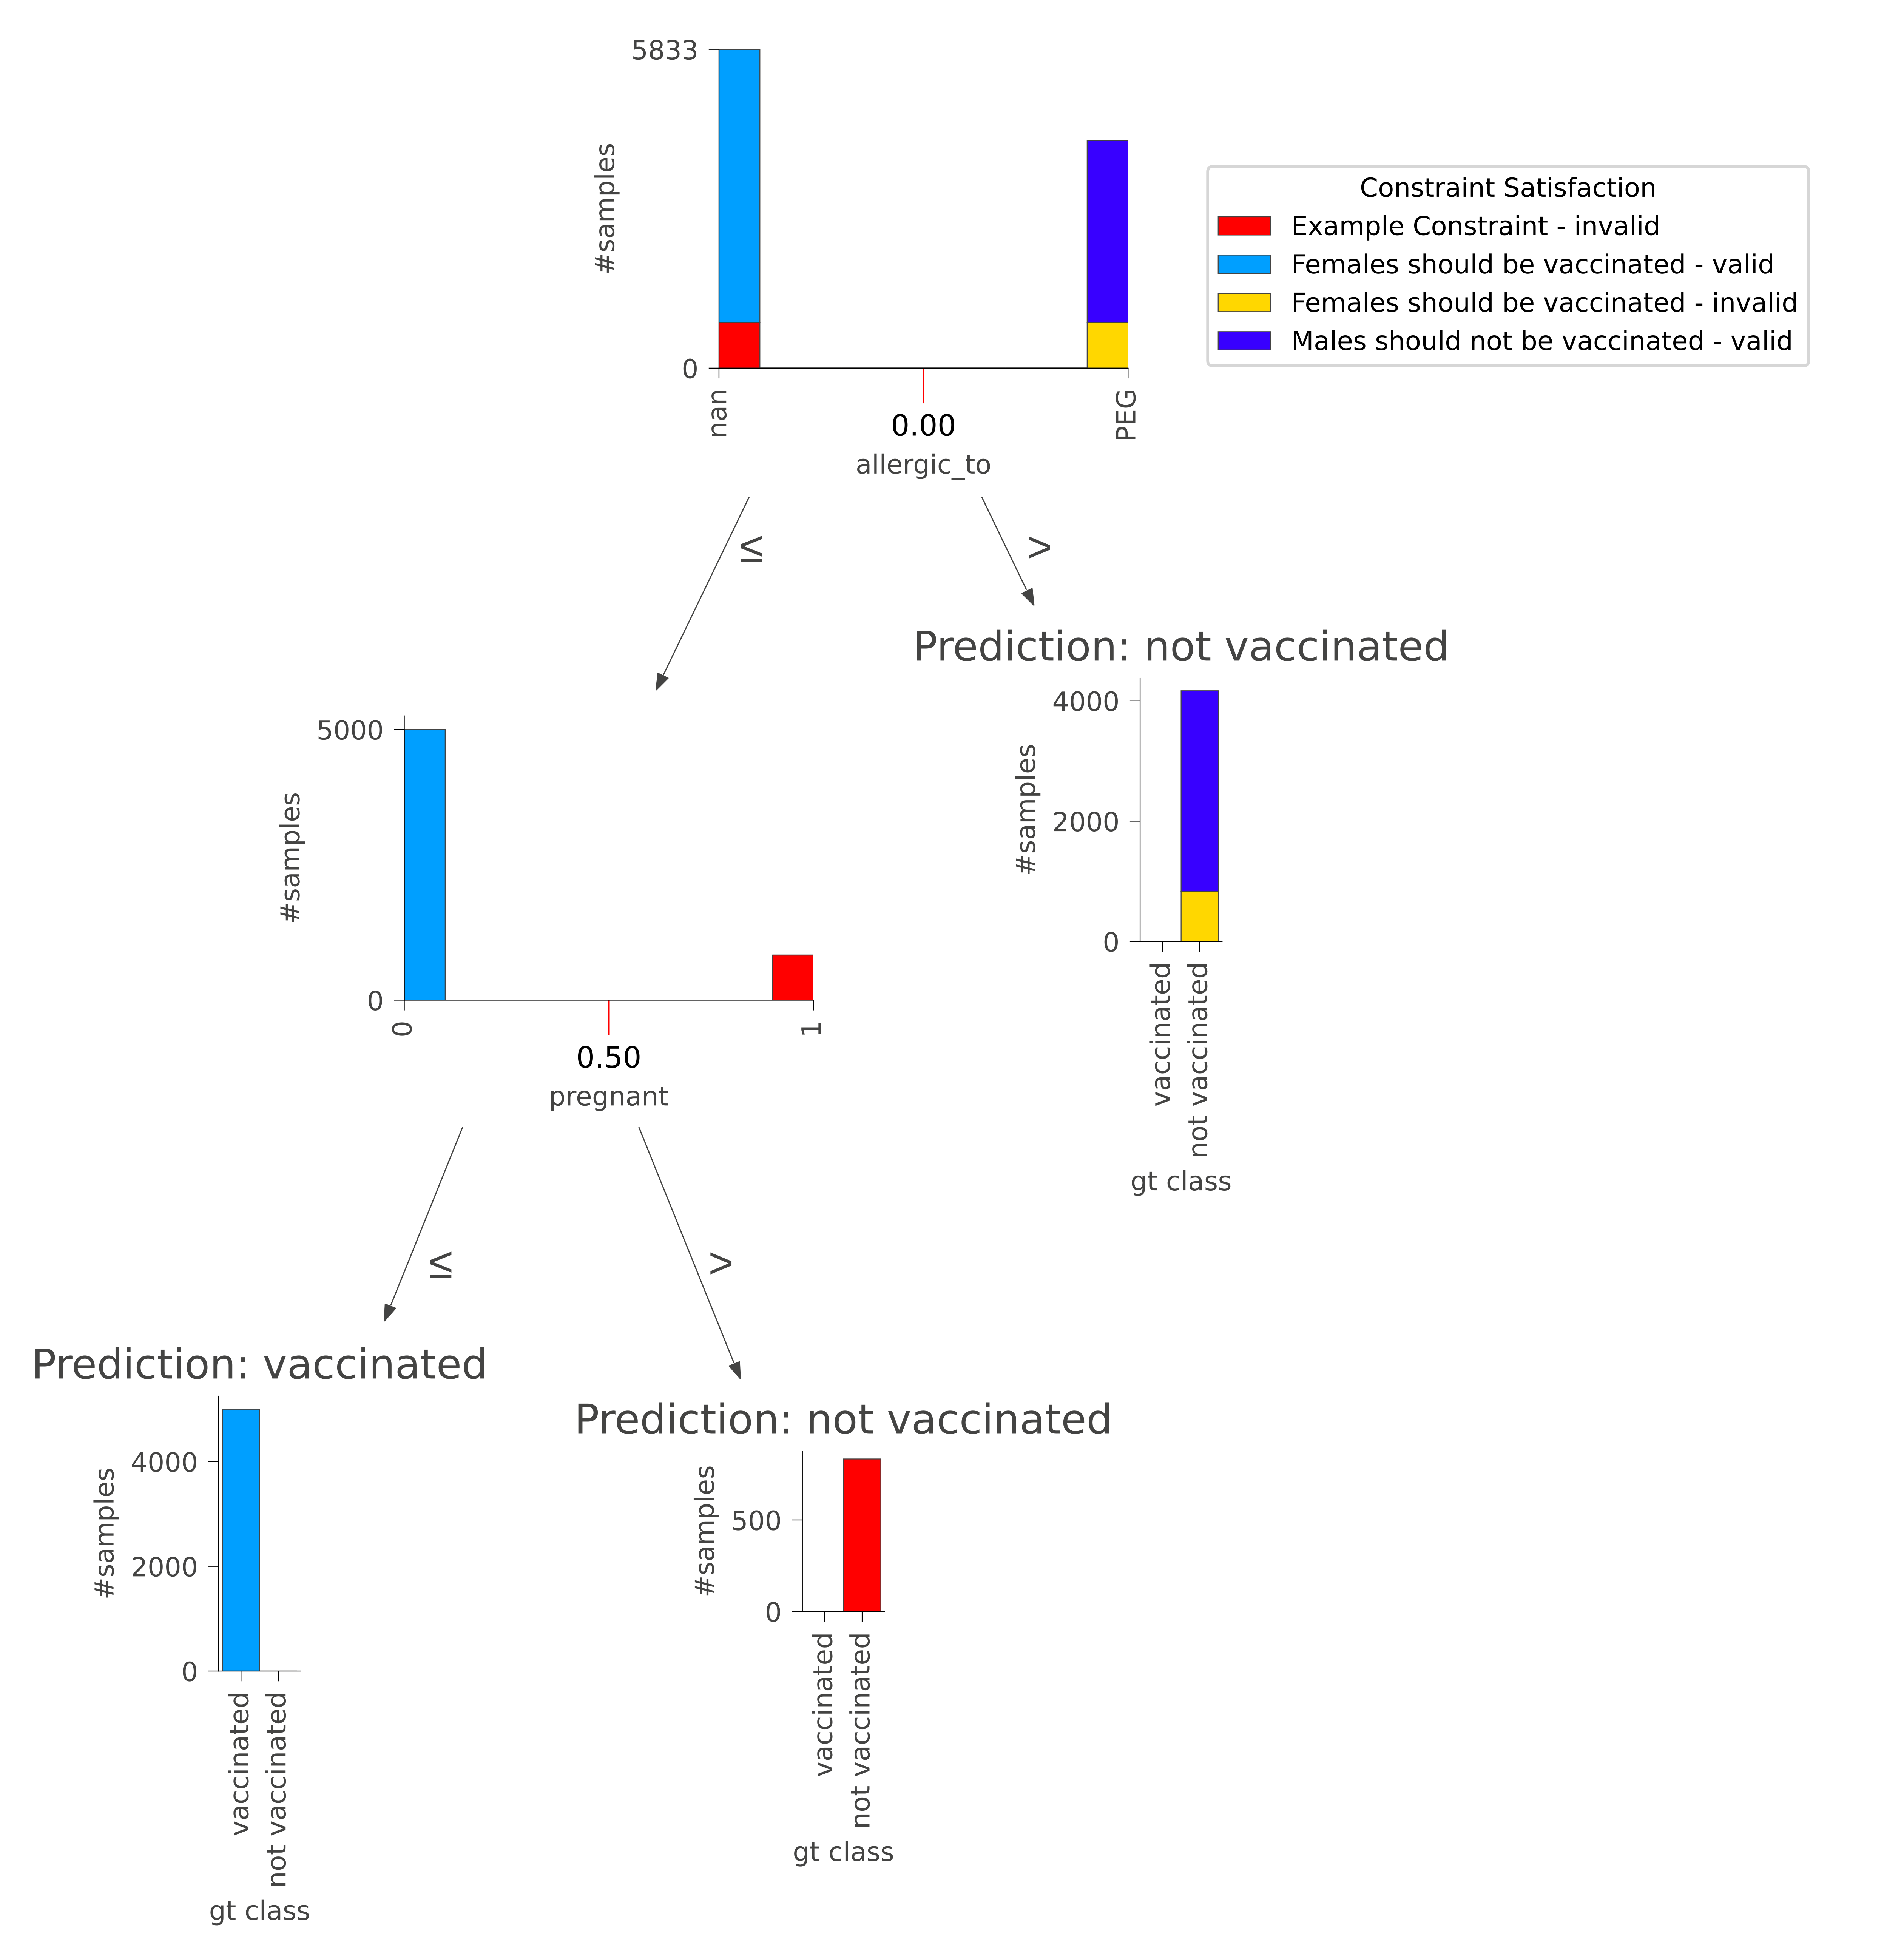
\includegraphics[scale=.07]{images/visualizations/Annotated Decision Tree Multiple Constraints gt grouping.png}    
            \captionof{figure}{Decision Tree of Figure \ref{motivating_example_decision_tree} annotated with the validation results from Figure \ref{fig:validation_results_summary_theta} and showing the ground truth class distributions in the leaves.}
            \label{fig:multiple_constraints_gt_annotated_motivating_example_decision_tree}
    \end{minipage}
\end{Bsp}



\paragraph{Additionally, Visualizing the Ground Truth Values of the Samples in Case of a Decision Tree Used for Regression}

In the case of a regression task, the ground truth values will be continuous, which allows to explicitly show the marginal effect the split features have on the precise ground truth value and the constraint validation result of a constraint. Therefore, the split node visualizations from Figure \ref{fig:sigmoid_dtree} can be reused and extended by choosing the colors of the samples in the scatter plot according to their constraint validation result (see Figure \ref{fig:constraint_viz_regression_tree}). 

However, this procedure only works for a single constraint and can be quite messy for large datasets. This is why the procedure described before can also be applied to the regression case; except for the grouping by the ground truth value.

\begin{figure}
    \centering
    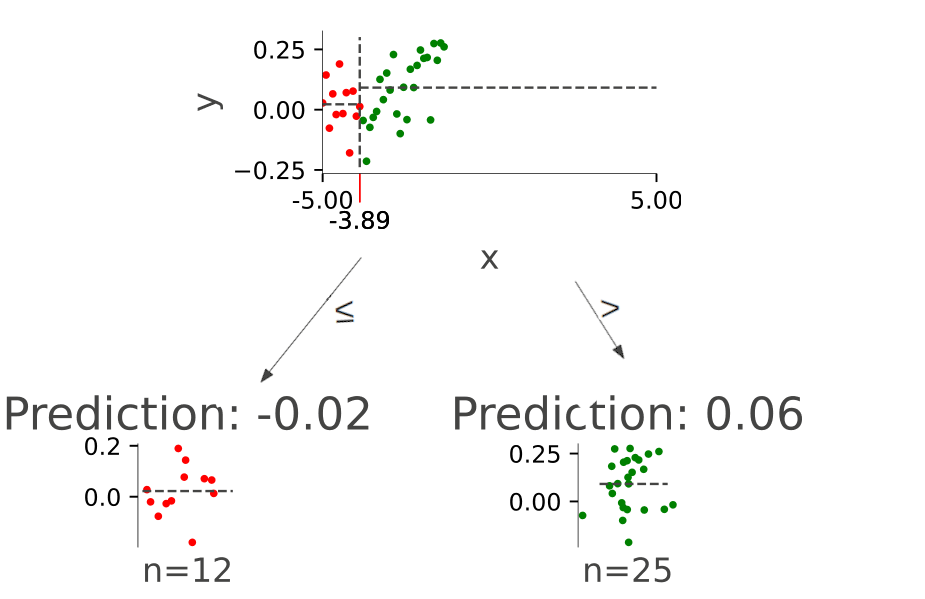
\includegraphics[width=0.6\textwidth]{images/visualizations/regression_tree_constraint.png}
    \caption{Showing the ground truth target values as in \ref{fig:sigmoid_dtree} while visualizing the constraint validation results. Red dots resp. green dots stand for invalidated resp. validated samples / predictions made on the basis of the samples}
    \label{fig:constraint_viz_regression_tree}
\end{figure}


\paragraph{Evaluating the Constraints per Decision Tree Node} Until this point, the model-validation-result function $\Theta$ was created by evaluating each constraint once for each sample $\mathbf{x}_i$, given the prediction $M_\theta(\mathbf{x}_i)$ of the decision tree. However, in the case of prediction constraints, it might be interesting to see the distribution of the validation results per node. For example, in section \ref{section_algorithms_performance_measures}, these distributions might have helped to choose the maximal depth of the decision tree, as over- and underfitting can be detected per node $n_{d,u}$ (i.e., using the interpretations from section \ref{section_confusion_matrix_decomposition}).



As each node in the decision tree is associated with a constant model $M_{c_{d,u}}$ (see section \ref{section_tree_based_models}), approaching the problem in lemma \ref{S:problem_explaining_ai_model_with_constraints} corresponds to solving multiple instances of the problem in lemma \ref{S:problem_validating_constraints_over_ai_model}. Each instance is associated with a node $n_{d,u}$ in the decision tree. Hence, the formulas \ref{formula_single_constraint_split} and \ref{formula_multiple_constraint_splits} need to use the model-validation-result function $\Theta_{M_{c_{d,u}},D,G,\eta}(C,i)$. This is in contrast to the formulas \ref{formula_single_constraint_leaf} and \ref{formula_multiple_constraints_leaf}, which can stay the same as the predictions made in the leaves of the decision tree correspond to the overall prediction the decision tree $M_\theta$ would make.
Luckily, the repeated evaluation of the same constraints over different models does not require the repeated evaluation of the SHACL shape schemas corresponding to the constraints, because the entity validation function \emph{validate} stays unchanged. Further, it turns out that it is enough to execute line \ref{algo:validation_engine:call_evaluateConstraints} (algorithm \ref{algo:validation_engine}) once for every occurring constant model prediction. This is for a group of constant models $M_{c_1}$,$M_{c_2}\hdots$ with $c_1 = c_2 = \hdots = c$ only $\Theta_{M_{c},D,G,\eta}$ is needed. In the case that these groups include all the constant models of the leave nodes, the evaluation of $\Theta_{M_{\theta},D,G,\eta}$ can be skipped. This limits the maximal amount of model-validation-result functions to the number of distinct predictions the model makes on the basis of the dataset used for the evaluation.

% \begin{Satz}{Minimizing the overhead of evaluating prediction constraints per decision tree node}{}
% The overhead of evaluating the prediction constraints $\mathcal{C} \subset \mathbf{C}$ per decision tree node is limited by the number of 
% \end{Satz}

\begin{Bsp}{Performing Node-based Constraint Validation}{node_based_constraint_validation}
    The motivating example is a binary classification problem. Therefore, only a maximum of two different model-validation-result functions should be needed. In the case of the motivating example decision tree, there are two different options. 
    First, one could use the model-validation-result function for the two possible classification results. The first group of constant models corresponding to the prediction \emph{vaccinated} would be, $\{M_{c_{1,1}}, M_{c_{2,1}}, M_{c_{3,1}}\}$ and the second group corresponding to \emph{not vaccinated} would be $\{M_{c_{2,2}}, M_{c_{3,2}}\}$. Clearly, the two groups cover each leaf and split node of the decision tree.
    The alternative used here is $\Theta_{M_{\theta},D,G,\eta}$ and $\Theta_{M_{\text{'vaccinated'}},D,G,\eta}$. The first function is used for all the leaf nodes and is already given in Figure \ref{fig:validation_results_summary_theta}. The second one is given below in Figure \ref{fig:validation_results_summary_theta_vaccinated} and is used for the split nodes.    
        
    % $\Theta_{M_{c_{1,1}},D,G,\eta}$ and $\Theta_{M_{c_{2,1}},D,G,\eta}$, which are based on the constant models $M_{c_{1,1}}$ and $M_{c_{2,1}}$ of the split nodes in figure \ref{motivating_example_decision_tree}. However $c_{1,1} = c_{2,1} = \text{'vaccinated'}$ and therefore $\Theta_{M_{c_{1,1}},D,G,\eta}(C,i) = \Theta_{M_{c_{2,1}},D,G,\eta}(C,i) = \Theta_{M_{\text{'vaccinated'}},D,G,\eta}(C,i)$ for all $i \in [1,...,N]$ and $C \in \mathbf{C}$.
    
    \captionsetup{type=htypei}
    \begin{minipage}[t]{\linewidth}
        \vspace{1ex}
        \centering
        \begin{tabular}{ll|ccc}
            \toprule
            dataset indices $i$ & Person & $\Theta(C,i)$ & $\Theta(C2,i)$ & $\Theta(C3,i)$\\
            \midrule
            \midrule
            $1...3333$     & \uri{:Max} & -1 & 0 & -1\\
            $3334...4166$  & \uri{:Maria} & 1 & -1 & 1\\
            $4167...9166$  & \uri{:Eva} & -1 & -1 & 1\\\
            $9167...9999$  & \uri{:Laura} & -1 & -1 & 1\\
            \bottomrule
        \end{tabular}
        \captionof{figure}{Table showing the model validation result function $\Theta_{M_{'vaccinated'},D,G,\eta}$ for the motivating example given the constraints $C$,$C2$ and $C3$}
        \label{fig:validation_results_summary_theta_vaccinated}
        \vspace{1ex}
    \end{minipage}
    
    % Secondly there is the  model-validation-result function $\Theta_{M_{\theta},G,\eta}$ needed for the leaves of the decision tree, which was already given in figure \ref{fig:validation_results_summary_theta}. 
    
    Using both model-validation-result functions (i.e., $\Theta_{M_{\theta},D,G,\eta}$ and $\Theta_{M_{\text{'vaccinated'}},D,G,\eta}$) the decision tree can be annotated with the constraint validation results per node (see Figure \ref{fig:multiple_constraints_per_node_annotated_motivating_example_decision_tree}) 
    
    The visualization is done based on the formulas \ref{formula_multiple_constraint_splits} (with $\Theta$ replaced with $\Theta_{M_{'vaccinated'},D,G,\eta}$) and \ref{formula_multiple_constraints_leaf}. Comparing the validation results of the newly created plot with Figure \ref{fig:multiple_constraints_gt_annotated_motivating_example_decision_tree} one can validate that only the validation results of the split nodes have changed. Further, the constant predictions (corresponding to the constant models used during the validation process), which would be made at a split nodes, if they were leaf nodes, are given above the plots. 
    
    In the case of the motivating example, it seems that the model could be improved by limiting the decision tree to a maximal depth of, $2$ as this is also according to the overfitting noted in example \ref{Bsp:composing_the_annotated_decision_tree}. Doing so would transform the node $n_{2,1}$ into a leave node and, therefore, all persons not allergic to \glqq PEG\grqq{} would get the recommendation to get vaccinated. This is in the sense of the example constraint, as it is evaluated to be valid for all samples in $R_{2,1}$ given.
    
        \captionsetup{type=htypei}
        \begin{minipage}[t]{\linewidth}
            \vspace{1ex}
            \centering
            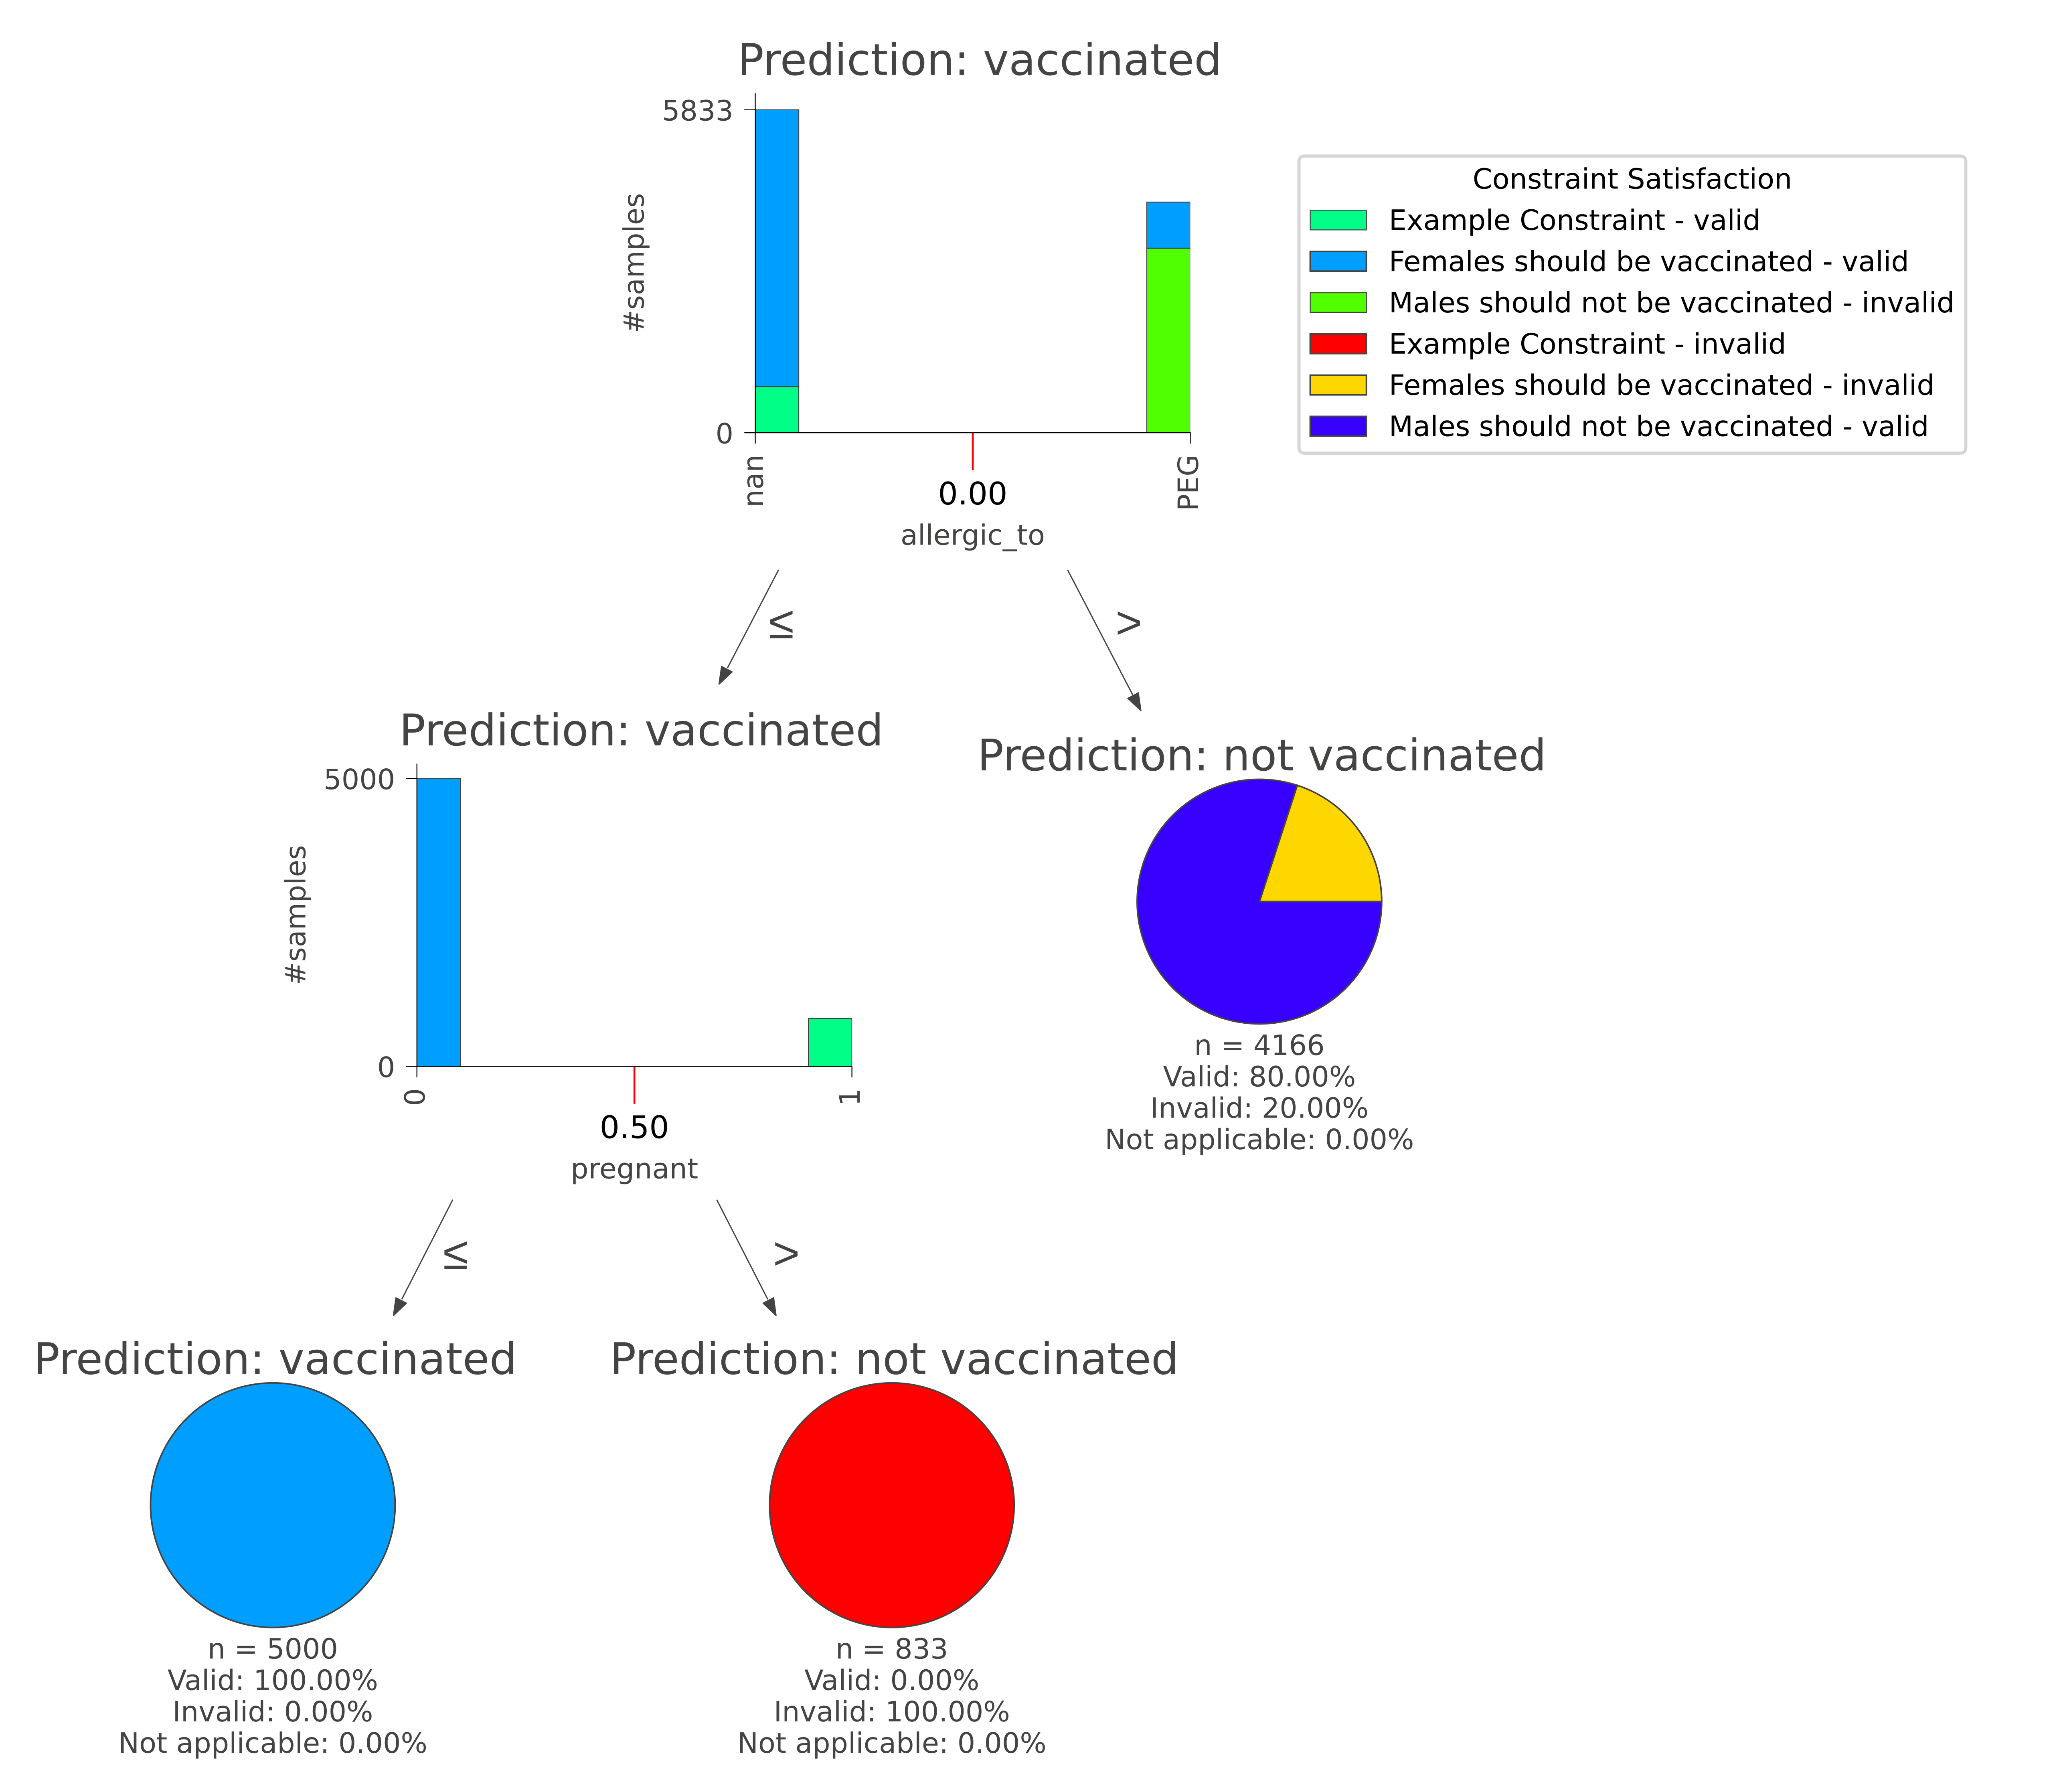
\includegraphics[scale=.07]{images/visualizations/Annotated Decision Tree per node predictions.png}    
            \captionof{figure}{Decision Tree of Figure \ref{motivating_example_decision_tree} annotated with the validation results calculated per node}
            \label{fig:multiple_constraints_per_node_annotated_motivating_example_decision_tree}
    \end{minipage}
\end{Bsp}